\documentclass[a4paper,11pt]{book}
\usepackage{makeidx}
\usepackage{graphicx}
\usepackage{amsfonts}
\usepackage{amssymb}
\usepackage{amsmath}
\usepackage{euscript}
\usepackage{boxedminipage}
\usepackage{lscape}
\usepackage{minitoc}
\usepackage{epsfig,psfrag,verbatim}
\usepackage{url,natbib}
\usepackage{booktabs, longtable}

\vfuzz2pt % Don't report over-full v-boxes if over-edge is small
\hfuzz2pt % Don't report over-full h-boxes if over-edge is small

\setlength{\oddsidemargin}{0cm}
\setlength{\evensidemargin}{0cm}
\setlength{\textwidth}{16cm}
\setlength{\textheight}{23cm}

\psdraft

\begin{document}
\title{Work package 9}
\author{}
\date{\today}
\maketitle
\tableofcontents

\subsubsection*{Acknowledgement}
This work was carried out in conjunction with the EURACE project (EU IST FP6
STREP grant 035086) which is a consortium lead by S. Cincotti (Universit\`{a} di
Genova), H. Dawid (Universitaet Bielefeld), C. Deissenberg (Universit\'{e} de la
M\'{e}diterran\'{e}e), K. Erkan (TUBITAK National Research Institute of Electronics
and Cryptology), M. Gallegati  (Universit\`{a} Politecnica delle Marche), M.
Holcombe (University of Sheffield), M. Marchesi (Universit\`{a} di Cagliari), C.
Greenough (STFC - Rutherford Appleton Laboratory).


\chapter{Innovation experiment}
%\input{Innovation_main}

\chapter{Energy shock experiment}

\section{Introduction}

As a benchmark, we first consider a situation in which there are no active
policy measures to counter the negative effects of an energy shock. This is the
benchmark scenario. We quantify the correlation between the level of the
energy shock and the change in GDP growth rate in this scenario.

We typically assume that an energy shock consists of a succession of
consecutive, identical (in length and magnitude) energy price increases.
Thus, an energy shock is captured by three parameters: the magnitude of the
single price increases ($\pi$), their periodicity $\Pi$ (the number of
days between two consecutive price increases), and the number of price
increases ($n).$ The total duration of the energy crisis ($d$) is then $%
d=\Pi n$. The price increase $\pi$ is assumed to instantaneously disappear at the end
of the total duration. The time profile of a typical energy shock is illustrated in Figure
\ref{Figure: energy shock} below.
We analyze the model response to variations to the three parameters duration
$d$, magnitude $\pi$, and periodicity $\Pi$.

\section{Description}

In the basic EURACE version, the investment goods producers update the price
of the investment good based on the increase in productivity of the
machinery. This reflects innovation and technological progress, which occurs
probabilistically. We now enrich the model by including the impact of the
energy costs on the investment goods.

The energy costs of the investment goods producers are incorporated into the
price of the capital good by an energy price mark-up equal to the magnitude
of the price shock ($\pi $):
\begin{equation}
p_{t+1}=(p_{t}+p_{t,c})(1+\pi ),
\end{equation}%
where($p_{t}$) is the price in period $t$ and ($p_{t,c}$) is the price
update due to the productivity increase.

The additional revenues stemming from the technologically motivated price
increase ($p_{t,c}$) are partly paid out as taxes and partly paid out as
dividends to households. BUT:\ HOW\ DO\ YOU\ COMPUTE\ THEM?\ A\ PRICE\
INCREASE\ NORMALLY\ HAS\ ALSO\ A\ QUANTITY\ EFFECT. THE\ QUANTITY\ EFFECT\
RESULTS\ BOTH\ FROM\ THE\ TECHNOLOGIACAL\ PRICE\ INCREASE\ AND\ FROM\ THE\
ENERGY\ PRICE\ INCREASE. HOW\ DO\ YOU\ UNTANGLE\ THAT?

The revenues that accrue due to the energy costs mark-up are not paid out in
taxes or dividends. Instead, the money is stored in a variable called %
\url{cum_energy_costs} that represents the total cumulative income of the
owners of the energy source (the Sheik of Qatar, Dubai, etc.), which does
not play any role in the EURACE dynamics. In other words, it leaves the
economic system decribed by EURACE.

\section{Experimental design}

In this section we describe how we setup the computational experiments.

\subsubsection*{Preliminaries.}

\bigskip We consider an energy shock over a pre-determined time interval $%
\left[ T_{a},T_{b}\right]$. The first, pre-shock $1000$ iterations are
ignored in the analysis of the experiment. Following these $1000$ initial
iterations, we run the model for $240$ further iterations before starting
the energy shock ($T_{a}=240$). After the energy shock period, at $t=T_{b}$,
we run the model for another $240$ iterations in order to analyze the legacy
of the shock. Thus, the total number of iterations for a single run (without
the transient period) is $240+(T_{b}-T_{a})+240$. To obtain statistically
significant results we perform $20$ batch runs per case (parameter
combination). See Table \ref{Table: experimental design} for details.

Figure \ref{Figure: energy shock} shows the time profile of such an
experiment. Figure \ref{Figure: empirical energy shock} shows the real
energy price behavior during the 2008 energy crisis. The price of Brent
crude oil went up by $+675\%$ between 2002.1-2008.6 (79 months), which
translates to a monthly increase of $2.45\%$. Then it went sharply down by $%
-70\%$ between 2008.7-2009.1 (7 months), which implies a monthly decrease of
$-5.8\%$.

\begin{figure}[th]
\centering\leavevmode
\begin{boxedminipage}{15cm}
\centering\leavevmode
\resizebox{7cm}{7cm}{% This file is generated by the MATLAB m-file laprint.m. It can be included
% into LaTeX documents using the packages epsfig and psfrag. It is accompanied
% by a postscript file. A sample LaTeX file is:
%    \documentclass{article} \usepackage{epsfig,psfrag}
%    \begin{document}\begin{figure}% This file is generated by the MATLAB m-file laprint.m. It can be included
% into LaTeX documents using the packages epsfig and psfrag. It is accompanied
% by a postscript file. A sample LaTeX file is:
%    \documentclass{article} \usepackage{epsfig,psfrag}
%    \begin{document}\begin{figure}\input{energy}\end{figure}\end{document}
% See http://www.uni-kassel.de/~linne/ for recent versions of laprint.m.
%
% created by:           LaPrint version 2.03 (19.1.2000)
% created on:           06-Oct-2009 10:58:03
% options used:         / noextrapicture
% latex width:          12 cm
% factor:               0.8
% eps file name:        energy.eps
% eps bounding box:     15 cm x 11.25 cm
% comment:              
%
\begin{psfrags}%
\psfragscanon%
%
% text strings:
\psfrag{str01}[t][t]{\sf Time (days)}%
\psfrag{str02}[t][t]{\sf Energy price}%
%
% xticklabels:
\psfrag{x01}[t][t]{0}%
\psfrag{x02}[t][t]{\sf 100}%
\psfrag{x03}[t][t]{\sf 200}%
\psfrag{x04}[t][t]{\sf 300}%
\psfrag{x05}[t][t]{\sf 400}%
\psfrag{x06}[t][t]{\sf 500}%
\psfrag{x07}[t][t]{\sf 600}%
%
% yticklabels:
\psfrag{v01}[r][r]{}%
\psfrag{v02}[r][r]{\sf $p_0$}%
\psfrag{v03}[r][r]{\sf $(1+\pi) p_0$}%
\psfrag{v04}[r][r]{\sf $(1+\pi)^2 p_0$}%
\psfrag{v05}[r][r]{}%
\psfrag{v06}[r][r]{}%
\psfrag{v07}[r][r]{}%
\psfrag{v08}[r][r]{}%
\psfrag{v09}[r][r]{}%
%
% Figure:
\resizebox{12cm}{!}{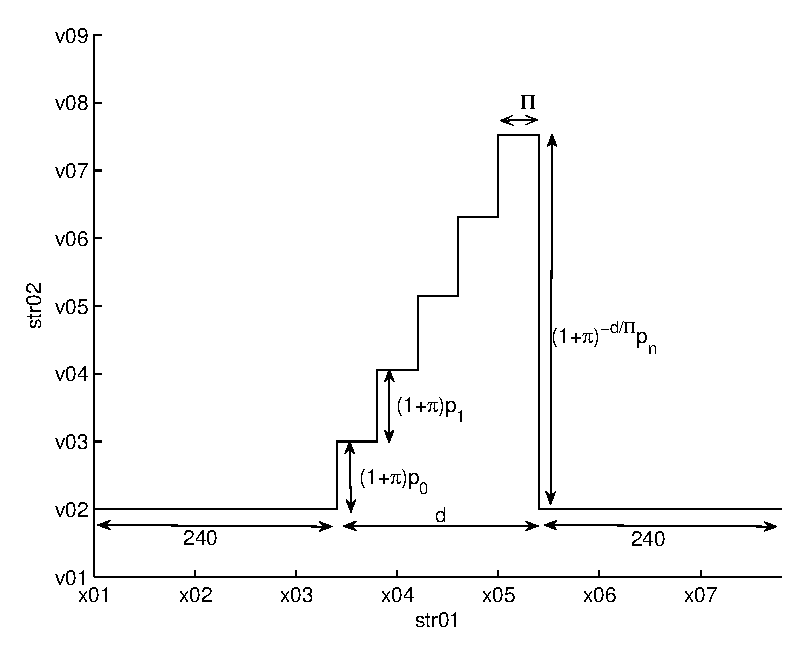
\epsfig{file=./energy_shock/eps/energy.eps}}%
\end{psfrags}%
%
% End energy.tex
\end{figure}\end{document}
% See http://www.uni-kassel.de/~linne/ for recent versions of laprint.m.
%
% created by:           LaPrint version 2.03 (19.1.2000)
% created on:           06-Oct-2009 10:58:03
% options used:         / noextrapicture
% latex width:          12 cm
% factor:               0.8
% eps file name:        energy.eps
% eps bounding box:     15 cm x 11.25 cm
% comment:              
%
\begin{psfrags}%
\psfragscanon%
%
% text strings:
\psfrag{str01}[t][t]{\sf Time (days)}%
\psfrag{str02}[t][t]{\sf Energy price}%
%
% xticklabels:
\psfrag{x01}[t][t]{0}%
\psfrag{x02}[t][t]{\sf 100}%
\psfrag{x03}[t][t]{\sf 200}%
\psfrag{x04}[t][t]{\sf 300}%
\psfrag{x05}[t][t]{\sf 400}%
\psfrag{x06}[t][t]{\sf 500}%
\psfrag{x07}[t][t]{\sf 600}%
%
% yticklabels:
\psfrag{v01}[r][r]{}%
\psfrag{v02}[r][r]{\sf $p_0$}%
\psfrag{v03}[r][r]{\sf $(1+\pi) p_0$}%
\psfrag{v04}[r][r]{\sf $(1+\pi)^2 p_0$}%
\psfrag{v05}[r][r]{}%
\psfrag{v06}[r][r]{}%
\psfrag{v07}[r][r]{}%
\psfrag{v08}[r][r]{}%
\psfrag{v09}[r][r]{}%
%
% Figure:
\resizebox{12cm}{!}{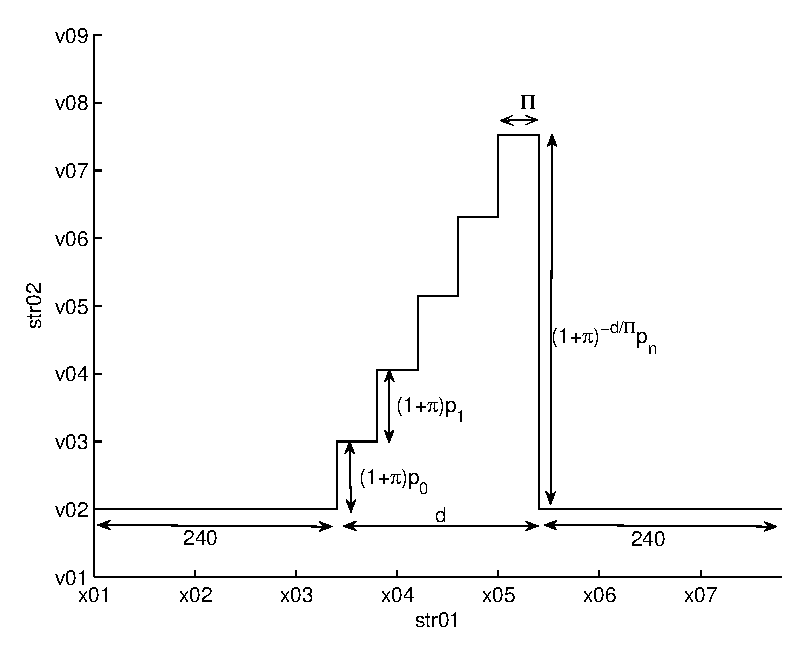
\epsfig{file=./energy_shock/eps/energy.eps}}%
\end{psfrags}%
%
% End energy.tex
}
\resizebox{7cm}{7cm}{% This file is generated by the MATLAB m-file laprint.m. It can be included
% into LaTeX documents using the packages epsfig and psfrag. It is accompanied
% by a postscript file. A sample LaTeX file is:
%    \documentclass{article} \usepackage{epsfig,psfrag}
%    \begin{document}\begin{figure}% This file is generated by the MATLAB m-file laprint.m. It can be included
% into LaTeX documents using the packages epsfig and psfrag. It is accompanied
% by a postscript file. A sample LaTeX file is:
%    \documentclass{article} \usepackage{epsfig,psfrag}
%    \begin{document}\begin{figure}\input{energy_single}\end{figure}\end{document}
% See http://www.uni-kassel.de/~linne/ for recent versions of laprint.m.
%
% created by:           LaPrint version 2.03 (19.1.2000)
% created on:           06-Oct-2009 11:24:53
% options used:         / noextrapicture
% latex width:          12 cm
% factor:               0.8
% eps file name:        energy_single.eps
% eps bounding box:     15 cm x 11.25 cm
% comment:              
%
\begin{psfrags}%
\psfragscanon%
%
% text strings:
\psfrag{str03}[t][t]{\sf Time (days)}%
\psfrag{str04}[b][b]{\sf Energy price}%
%
% xticklabels:
\psfrag{x01}[t][t]{\sf 0}%
\psfrag{x02}[t][t]{\sf 100}%
\psfrag{x03}[t][t]{\sf 200}%
\psfrag{x04}[t][t]{\sf 300}%
\psfrag{x05}[t][t]{\sf 400}%
\psfrag{x06}[t][t]{\sf 500}%
\psfrag{x07}[t][t]{\sf 600}%
%
% yticklabels:
\psfrag{v01}[r][r]{}%
\psfrag{v02}[r][r]{\sf $p_0$}%
\psfrag{v03}[r][r]{\sf $(1+\pi) p_0$}%
\psfrag{v04}[r][r]{}%
\psfrag{v05}[r][r]{}%
\psfrag{v06}[r][r]{}%
\psfrag{v07}[r][r]{}%
\psfrag{v08}[r][r]{}%
\psfrag{v09}[r][r]{}%
%
% Figure:
\resizebox{12cm}{!}{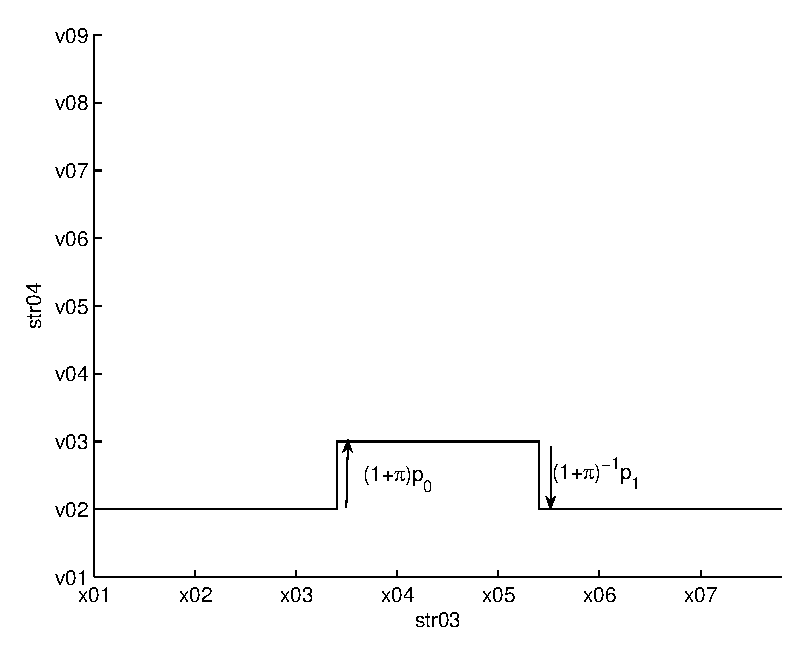
\epsfig{file=./energy_shock/eps/energy_single.eps}}%
\end{psfrags}%
%
% End energy_single.tex
\end{figure}\end{document}
% See http://www.uni-kassel.de/~linne/ for recent versions of laprint.m.
%
% created by:           LaPrint version 2.03 (19.1.2000)
% created on:           06-Oct-2009 11:24:53
% options used:         / noextrapicture
% latex width:          12 cm
% factor:               0.8
% eps file name:        energy_single.eps
% eps bounding box:     15 cm x 11.25 cm
% comment:              
%
\begin{psfrags}%
\psfragscanon%
%
% text strings:
\psfrag{str03}[t][t]{\sf Time (days)}%
\psfrag{str04}[b][b]{\sf Energy price}%
%
% xticklabels:
\psfrag{x01}[t][t]{\sf 0}%
\psfrag{x02}[t][t]{\sf 100}%
\psfrag{x03}[t][t]{\sf 200}%
\psfrag{x04}[t][t]{\sf 300}%
\psfrag{x05}[t][t]{\sf 400}%
\psfrag{x06}[t][t]{\sf 500}%
\psfrag{x07}[t][t]{\sf 600}%
%
% yticklabels:
\psfrag{v01}[r][r]{}%
\psfrag{v02}[r][r]{\sf $p_0$}%
\psfrag{v03}[r][r]{\sf $(1+\pi) p_0$}%
\psfrag{v04}[r][r]{}%
\psfrag{v05}[r][r]{}%
\psfrag{v06}[r][r]{}%
\psfrag{v07}[r][r]{}%
\psfrag{v08}[r][r]{}%
\psfrag{v09}[r][r]{}%
%
% Figure:
\resizebox{12cm}{!}{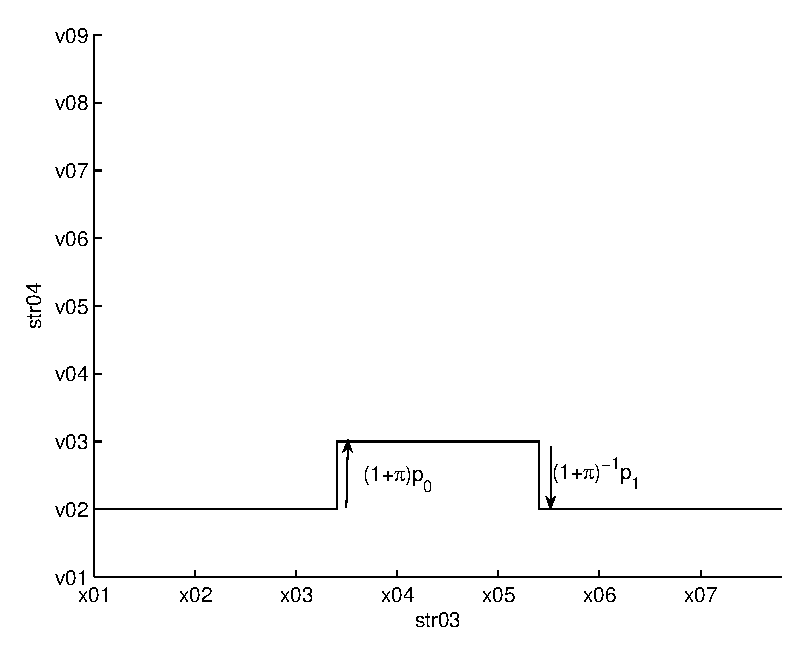
\epsfig{file=./energy_shock/eps/energy_single.eps}}%
\end{psfrags}%
%
% End energy_single.tex
}
\end{boxedminipage}
\caption{The time profile of an energy shock experiment. Left panel:
periodicity $0<\Pi<+\infty $, right panel: periodicity $\Pi=+\infty $.}
\label{Figure: energy shock}
\end{figure}

\begin{figure}[ht!]
\centering\leavevmode
\begin{boxedminipage}{10.5cm}
\centering\leavevmode
\resizebox{10cm}{7cm}{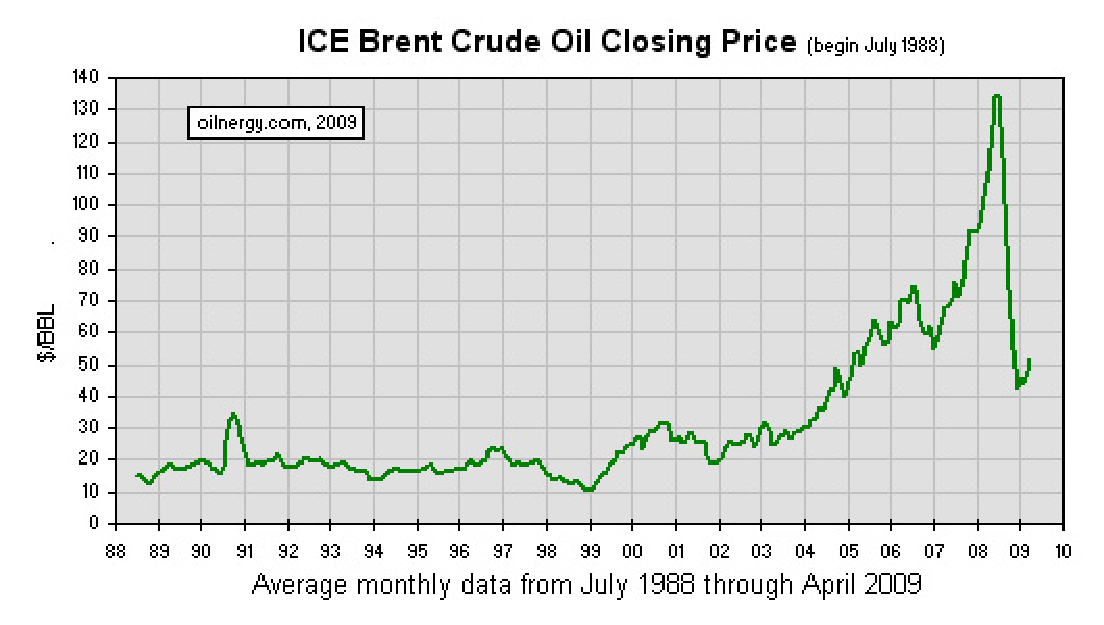
\includegraphics{./energy_shock/eps/Brent_1988_2009.eps}}
\end{boxedminipage}
\caption{Empirical energy prices during the 2008 energy crisis. An increase
of $2.45\%$ per month over a period of 79 months ($+675\%$), followed by a
sharp decline of $-5.8\%$ per month during 7 months ($-70\%$).}
\label{Figure: empirical energy shock}
\end{figure}

We consider the following values of $d$:
\begin{itemize}
\item Short energy crisis scenario: $d=40$ days,
\item Long energy crisis scenario: $d=240$ days,
\end{itemize}
and for each of these two values the following cases:

\begin{itemize}
\item Case 1: periodicity $\Pi=0$
\end{itemize}

There is a single instantaneous energy price increase $\pi$ at $T_{a},$ and
an instantaneous decrease of the same magnitude at $T_{b}.$ However, in the
meantime the capital goods price is updated as usual with the productivity
progress, so the price of the investment goods at $T_{b}$ will nonetheless
differ from their price level at $T_{a}$.

\begin{itemize}
\item Case 2: periodicity $\Pi>0$

\item There are $n$ consecutive instantaneous price increases between $T_{a}$
and $T_{b}$, at equidistant time intervals, and an instantaneous decrease
of magnitude $(1+\pi)^{-n}$ in $T_{b}$. This brings the price back to its pre-shock level, 
if no other influences affected the price in the meantime.
\end{itemize}

Table \ref{Table: parameter settings} gives the parameter values used in the
computational experiments, and Table \ref{Table: computational setting} summarizes the computational
setting.

\begin{table}[tbp]
\caption{Parameter values}
\centering
\begin{tabular}{llll}
\hline\hline
Name & Symbol & Values & Description \\ \hline
duration & $d$ & $240$ & Duration of the energy crisis in days \\
intensity & $\pi$ & $\{0.01, 0.05\}$ & Percentage price change for a
single shock \\
periodicity & $\Pi$ & $\{20, +\infty\}$ & Periodicity of the shock in days%
\end{tabular}%
\label{Table: parameter settings}
\end{table}

\begin{table}[tbp]
\caption{Overview of the computational setting.}
\label{Table: computational setting}
\centering
\begin{tabular}{ll}
\hline\hline
Name & Value \\ \hline
Cases & $18$ \\
Batch runs per case & $20$ \\
Iterations per run & $300$ \\
Pre-iterations & $1000$ \\ \hline
\end{tabular}%
\end{table}

\section{Simulations}
We focus our analysis on the four cases in Table \ref{Table: parameter settings}.
The duration of the energy crisis is always $240$ days (1 year), and we
have either a periodicity of $20$ days or a single shock at the beginning and a single shock downward at the end.

We recall the benchmark results in Fig. \ref{Figure: benchmark}: GDP settles down to a stable growth path, the unemployment rate is stable as well, and the capital goods price shows a characteristic staircase.

In Figure \ref{Figure: energy shock 1} we introduce a mild energy shock of $1\%$ at iteration $1240$.
After $240$ days there is a downward shock of $1\%$. As can be seen from the figure there is a small blip in the capital goods price (Fig. \ref{Figure: energy shock 1}c), but this has hardly any effect on the economy.

Figure \ref{Figure: energy shock 2} shows a single shock of $5\%$, and a symmetric downward shock at the end.
For one year the capital goods price is significantly increased, but still this does not have any significant effect on key macroeconomic variables such as GDP and the unemployment rate.

A more prolonged energy crisis is shown in Figure \ref{Figure: energy shock 3}, where there are multiple shocks of $1\%$, one every $20$ days. This results in a more pronounced energy spike, as can be seen in Fig. \ref{Figure: energy shock 3}c. But the effect on GDP and the unemployment rate remains relatively minor. 
We also show the daily energy costs that are accumulated during the energy crisis (Fig. \ref{Figure: energy shock 3}d). The unemployment rate goes down during the energy crisis, which can be explained due to the substitution effect of labour for capital.

The final case is the one shown in Figure \ref{Figure: energy shock 4} where we have multiple shocks of $5\%$, one every $20$ days. Here finally we have the signature of a true energy crisis, where at its peak capital goods cost 3 times as much as it did at the start of the crisis. The downward effect on GDP and unemployment is pronounced.

This case will now be used in the next section, where we introduce a macroeconomic stabilization policy to mitigate the effects of such a negative shock to the economy.
 %4 pages
%\begin{comment}
\clearpage
\pagebreak
\pagebreak
\pagebreak
\pagebreak
\begin{comment}
\documentclass{article}
\usepackage{epsfig,graphicx,verbatim, boxedminipage, url}
\begin{document}
%\subsubsection*{EURACE Energy shock experiment}
%\today
This version: October 12, 2009\\
Model used: EURACE Integrated Model, rev 2800, October 10, 2009\\
\end{comment}

\subsubsection*{Benchmark Scenario}
\begin{figure}[ht!]
\centering\leavevmode
\begin{minipage}{16cm}
\centering\leavevmode
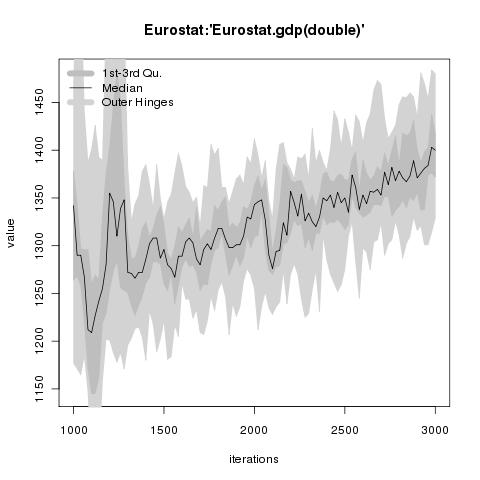
\includegraphics[width=5cm]{./energy_shock/bench/Eurostat-gdp.png}
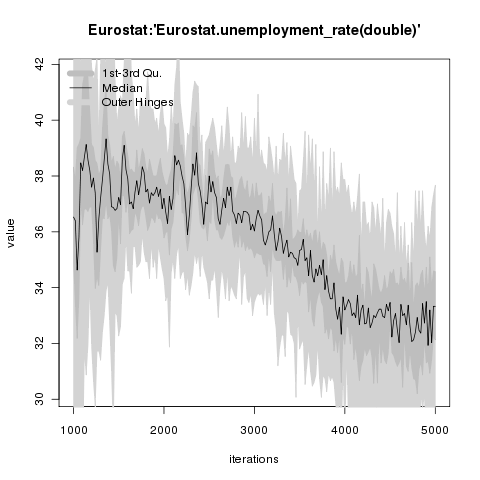
\includegraphics[width=5cm]{./energy_shock/bench/Eurostat-unemployment_rate.png}
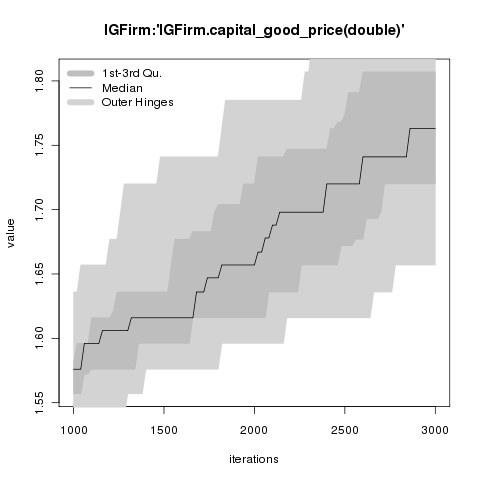
\includegraphics[width=5cm]{./energy_shock/bench/IGFirm-capital_good_price.png}
\end{minipage}
\caption{Benchmark scenario for the energy shock experiment. The capital good price, GDP and unemployment rate.}
\label{Figure: benchmark}
\end{figure}
%\pagebreak

\begin{figure}[ht!]
\centering\leavevmode
\begin{minipage}{17cm}
\centering\leavevmode
{$d=240, \pi=0.01, \Pi=0$}\\
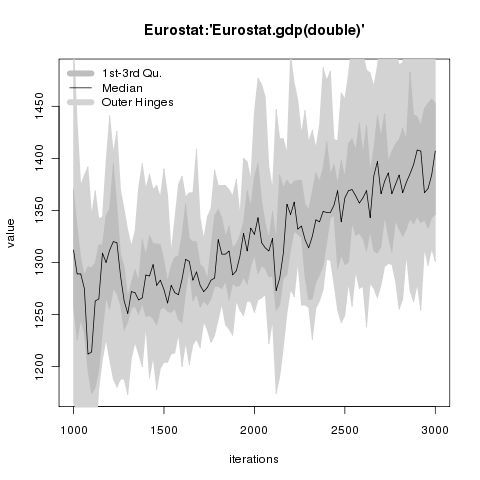
\includegraphics[width=5cm]{./energy_shock/png/duration_240/intensity_0.01/frequency_0/Eurostat-gdp.png}
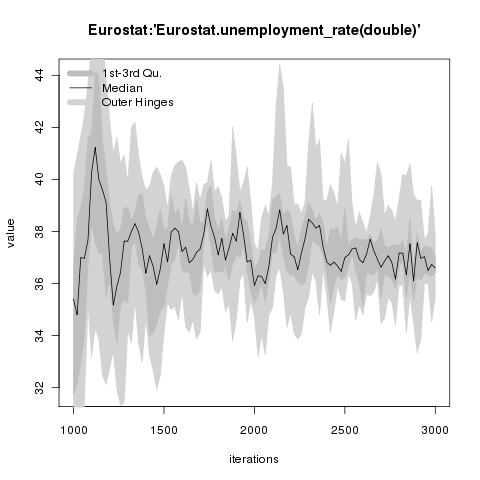
\includegraphics[width=5cm]{./energy_shock/png/duration_240/intensity_0.01/frequency_0/Eurostat-unemployment_rate.png}
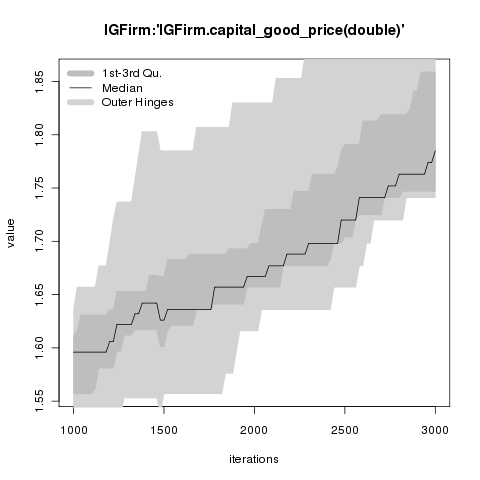
\includegraphics[width=5cm]{./energy_shock/png/duration_240/intensity_0.01/frequency_0/IGFirm-capital_good_price.png}
\end{minipage}
\caption{Energy shock parameters: duration $d=240$, intensity $\pi=0.01$, periodicity $\Pi=0$.}
\label{Figure: energy shock 1}
\end{figure}

\begin{figure}[ht!]
\centering\leavevmode
\begin{minipage}{17cm}
\centering\leavevmode
{$d=240, \pi=0.05, \Pi=0$}\\
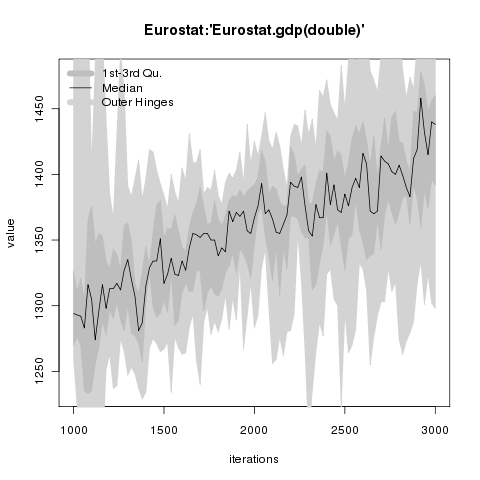
\includegraphics[width=5cm]{./energy_shock/png/duration_240/intensity_0.05/frequency_0/Eurostat-gdp.png}
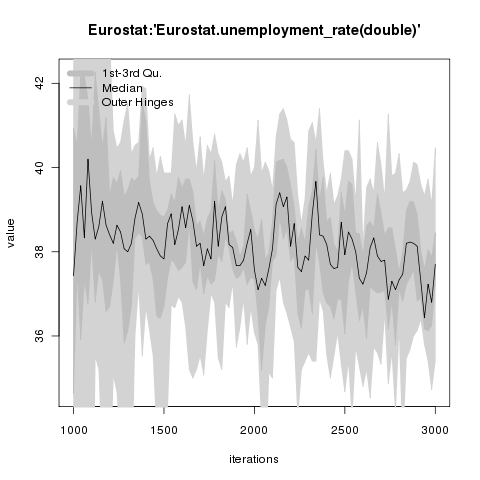
\includegraphics[width=5cm]{./energy_shock/png/duration_240/intensity_0.05/frequency_0/Eurostat-unemployment_rate.png}
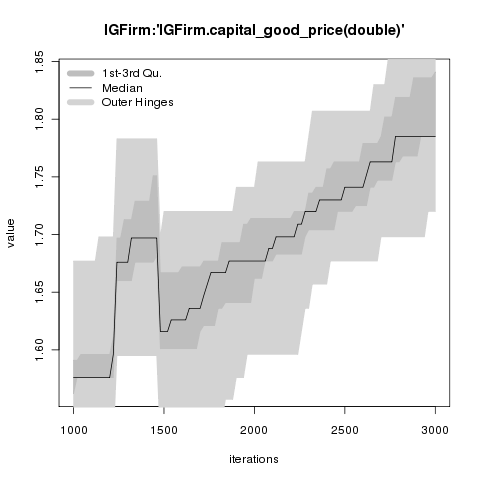
\includegraphics[width=5cm]{./energy_shock/png/duration_240/intensity_0.05/frequency_0/IGFirm-capital_good_price.png}
\end{minipage}
\caption{Energy shock parameters: duration $d=240$, intensity $\pi=0.05$, periodicity $\Pi=0$.}
\label{Figure: energy shock 2}
\end{figure}

\begin{figure}[ht!]
\centering\leavevmode
\begin{minipage}{17cm}
\centering\leavevmode
{$d=240, \pi=0.01, \Pi=20$}\\
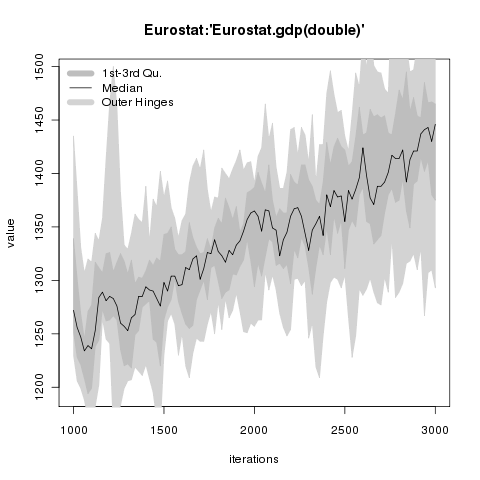
\includegraphics[width=8cm]{./energy_shock/png/duration_240/intensity_0.01/frequency_20/Eurostat-gdp.png}
\includegraphics[width=8cm]{./energy_shock/png/duration_240/intensity_0.01/frequency_20/Eurostat-unemployment_rate.png}
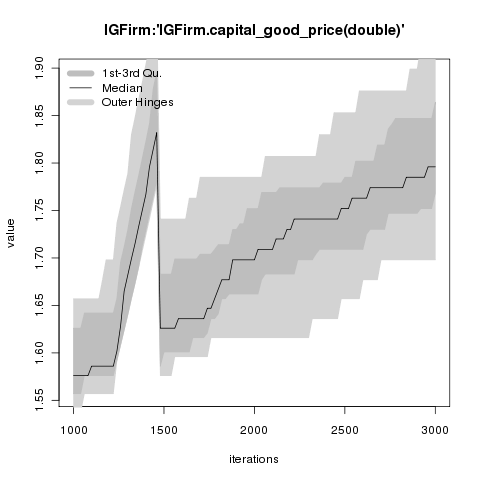
\includegraphics[width=8cm]{./energy_shock/png/duration_240/intensity_0.01/frequency_20/IGFirm-capital_good_price.png}
\includegraphics[width=8cm]{./energy_shock/png/duration_240/intensity_0.01/frequency_20/IGFirm-energy_costs_per_day.png}
\end{minipage}
\caption{Energy shock parameters: duration $d=240$, intensity $\pi=0.01$, periodicity $\Pi=20$.}
\label{Figure: energy shock 3}
\end{figure}

\begin{figure}[ht!]
\centering\leavevmode
\begin{minipage}{17cm}
\centering\leavevmode
{$d=240, \pi=0.05, \Pi=20$}\\
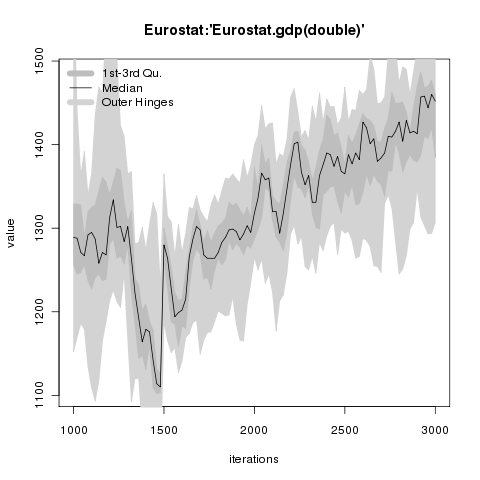
\includegraphics[width=8cm]{./energy_shock/png/duration_240/intensity_0.05/frequency_20/Eurostat-gdp.png}
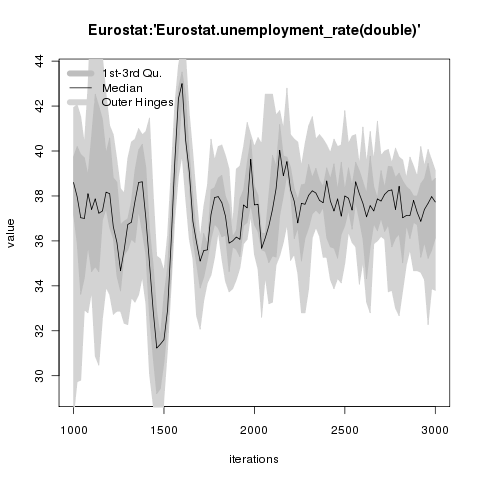
\includegraphics[width=8cm]{./energy_shock/png/duration_240/intensity_0.05/frequency_20/Eurostat-unemployment_rate.png}
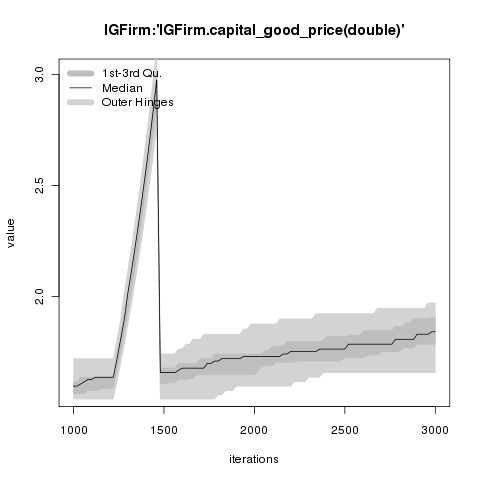
\includegraphics[width=8cm]{./energy_shock/png/duration_240/intensity_0.05/frequency_20/IGFirm-capital_good_price.png}
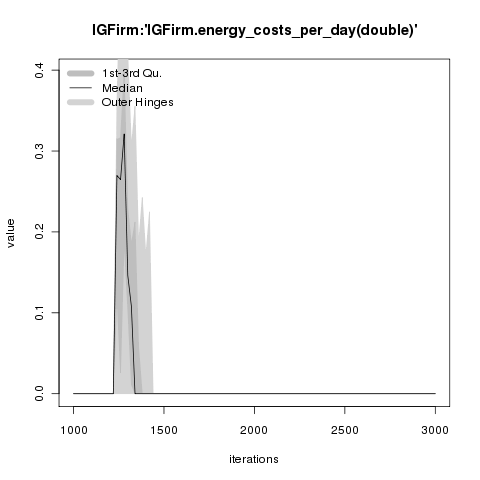
\includegraphics[width=8cm]{./energy_shock/png/duration_240/intensity_0.05/frequency_20/IGFirm-energy_costs_per_day.png}
\end{minipage}
\caption{Energy shock parameters: duration $d=240$, intensity $\pi=0.05$, periodicity $\Pi=20$.}
\label{Figure: energy shock 4}
\end{figure}


%\end{document}
\begin{comment}
%\begin{figure}[ht!]
\centering\leavevmode
\begin{minipage}{13cm}
\centering\leavevmode
{$d=240, \pi=0.05, \Pi=20$}\\
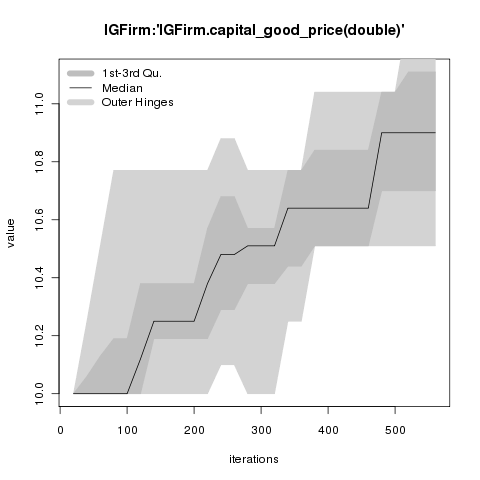
\includegraphics[width=6cm]{./png/duration_240/intensity_0.05/frequency_20/IGFirm-capital_good_price.png}
\includegraphics[width=6cm]{./png/duration_240/intensity_0.05/frequency_20/IGFirm-energy_costs_per_day.png}
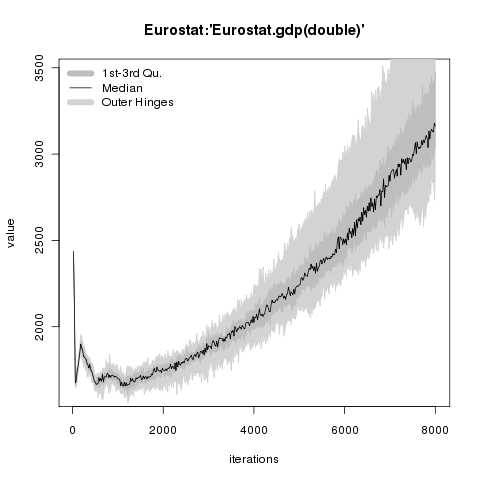
\includegraphics[width=6cm]{./png/duration_240/intensity_0.05/frequency_20/Eurostat-gdp.png}
\includegraphics[width=6cm]{./png/duration_240/intensity_0.05/frequency_20/Eurostat-unemployment_rate.png}
\end{minipage}
%\caption{Energy shock parameters: duration $d=240$, intensity $\pi=0.05, periodicity $\Pi=20$.}
%\label{Figure: IGFirm-capital_good_price}
\end{figure}

%\ref{Figure: energy shock 1}
%\begin{figure}[ht!]
\centering\leavevmode
\begin{minipage}{13cm}
\centering\leavevmode
{$d=240, \pi=0.05, \Pi=20$}\\
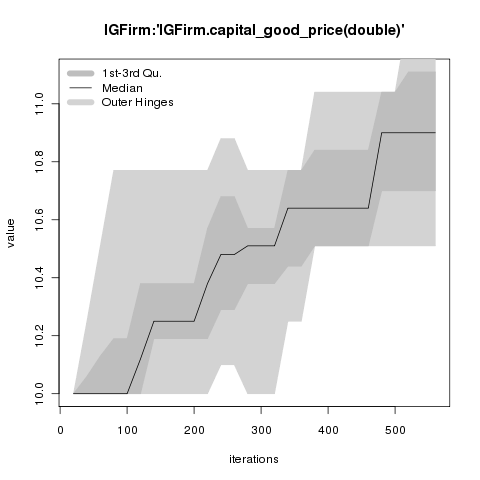
\includegraphics[width=6cm]{./png/duration_240/intensity_0.05/frequency_20/IGFirm-capital_good_price.png}
\includegraphics[width=6cm]{./png/duration_240/intensity_0.05/frequency_20/IGFirm-energy_costs_per_day.png}
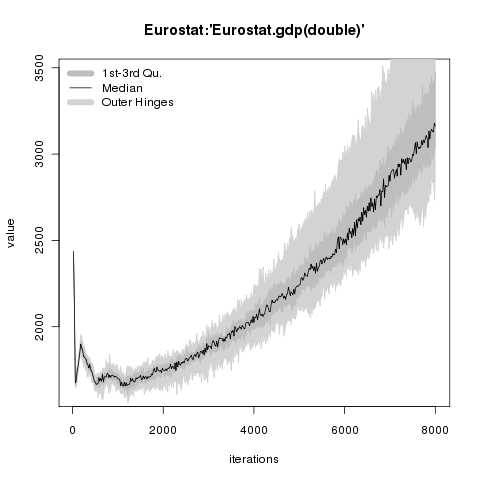
\includegraphics[width=6cm]{./png/duration_240/intensity_0.05/frequency_20/Eurostat-gdp.png}
\includegraphics[width=6cm]{./png/duration_240/intensity_0.05/frequency_20/Eurostat-unemployment_rate.png}
\end{minipage}
%\caption{Energy shock parameters: duration $d=240$, intensity $\pi=0.05, periodicity $\Pi=20$.}
%\label{Figure: IGFirm-capital_good_price}
\end{figure}

%\ref{Figure: energy shock 2}
%\begin{figure}[ht!]
\centering\leavevmode
\begin{minipage}{13cm}
\centering\leavevmode
{$d=240, \pi=0.05, \Pi=20$}\\
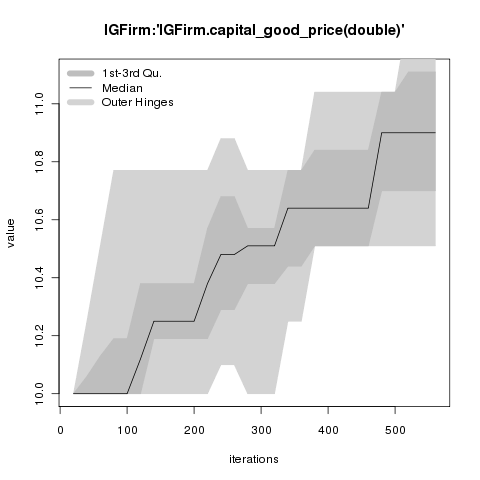
\includegraphics[width=6cm]{./png/duration_240/intensity_0.05/frequency_20/IGFirm-capital_good_price.png}
\includegraphics[width=6cm]{./png/duration_240/intensity_0.05/frequency_20/IGFirm-energy_costs_per_day.png}
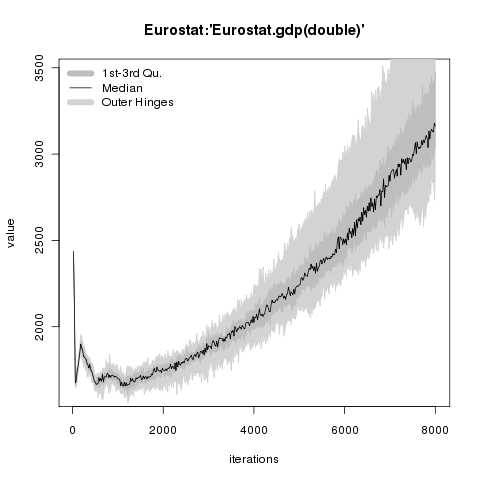
\includegraphics[width=6cm]{./png/duration_240/intensity_0.05/frequency_20/Eurostat-gdp.png}
\includegraphics[width=6cm]{./png/duration_240/intensity_0.05/frequency_20/Eurostat-unemployment_rate.png}
\end{minipage}
%\caption{Energy shock parameters: duration $d=240$, intensity $\pi=0.05, periodicity $\Pi=20$.}
%\label{Figure: IGFirm-capital_good_price}
\end{figure}

%\ref{Figure: energy shock 3}
%\begin{figure}[ht!]
\centering\leavevmode
\begin{minipage}{13cm}
\centering\leavevmode
{$d=240, \pi=0.05, \Pi=20$}\\
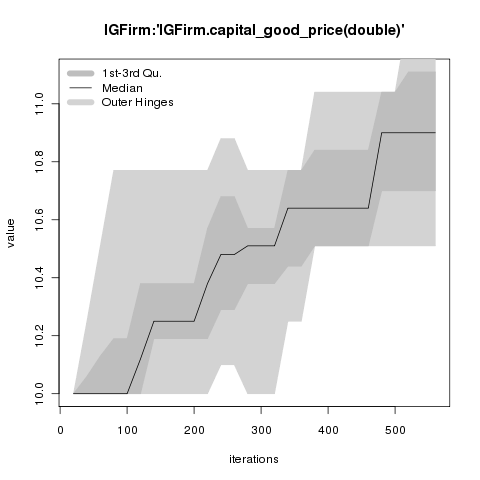
\includegraphics[width=6cm]{./png/duration_240/intensity_0.05/frequency_20/IGFirm-capital_good_price.png}
\includegraphics[width=6cm]{./png/duration_240/intensity_0.05/frequency_20/IGFirm-energy_costs_per_day.png}
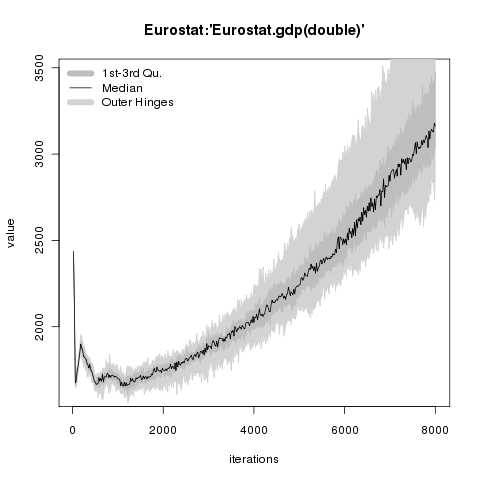
\includegraphics[width=6cm]{./png/duration_240/intensity_0.05/frequency_20/Eurostat-gdp.png}
\includegraphics[width=6cm]{./png/duration_240/intensity_0.05/frequency_20/Eurostat-unemployment_rate.png}
\end{minipage}
%\caption{Energy shock parameters: duration $d=240$, intensity $\pi=0.05, periodicity $\Pi=20$.}
%\label{Figure: IGFirm-capital_good_price}
\end{figure}

%\ref{Figure: energy shock 4}

%\subsubsection*{Duration $40$, intensity $1\%$, frequency $\{0,20,60\}$}
\begin{figure}[ht!]
\centering\leavevmode
\begin{minipage}{13cm}
\centering\leavevmode
{$d=240, \pi=0.05, \Pi=20$}\\
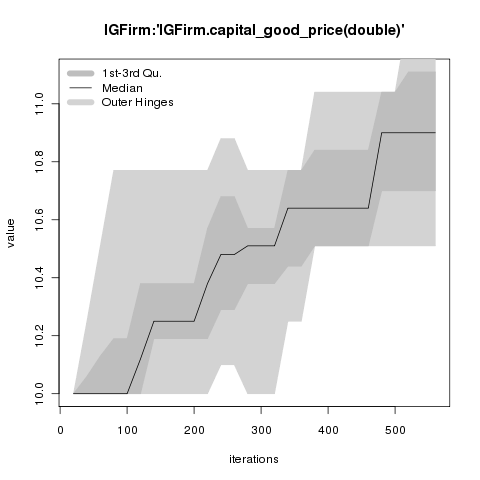
\includegraphics[width=6cm]{./png/duration_240/intensity_0.05/frequency_20/IGFirm-capital_good_price.png}
\includegraphics[width=6cm]{./png/duration_240/intensity_0.05/frequency_20/IGFirm-energy_costs_per_day.png}
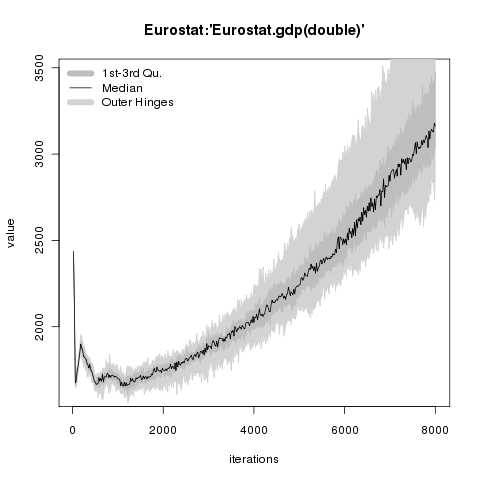
\includegraphics[width=6cm]{./png/duration_240/intensity_0.05/frequency_20/Eurostat-gdp.png}
\includegraphics[width=6cm]{./png/duration_240/intensity_0.05/frequency_20/Eurostat-unemployment_rate.png}
\end{minipage}
%\caption{Energy shock parameters: duration $d=240$, intensity $\pi=0.05, periodicity $\Pi=20$.}
%\label{Figure: IGFirm-capital_good_price}
\end{figure}


\begin{figure}[ht!]
\centering\leavevmode
\begin{minipage}{13cm}
\centering\leavevmode
{$d=240, \pi=0.05, \Pi=20$}\\
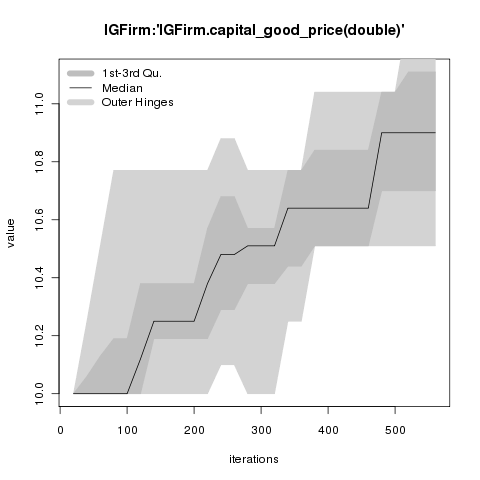
\includegraphics[width=6cm]{./png/duration_240/intensity_0.05/frequency_20/IGFirm-capital_good_price.png}
\includegraphics[width=6cm]{./png/duration_240/intensity_0.05/frequency_20/IGFirm-energy_costs_per_day.png}
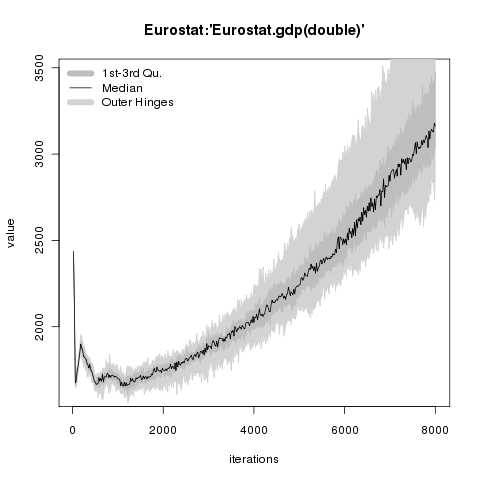
\includegraphics[width=6cm]{./png/duration_240/intensity_0.05/frequency_20/Eurostat-gdp.png}
\includegraphics[width=6cm]{./png/duration_240/intensity_0.05/frequency_20/Eurostat-unemployment_rate.png}
\end{minipage}
%\caption{Energy shock parameters: duration $d=240$, intensity $\pi=0.05, periodicity $\Pi=20$.}
%\label{Figure: IGFirm-capital_good_price}
\end{figure}


%\begin{figure}[ht!]
\centering\leavevmode
\begin{minipage}{13cm}
\centering\leavevmode
{$d=240, \pi=0.05, \Pi=20$}\\
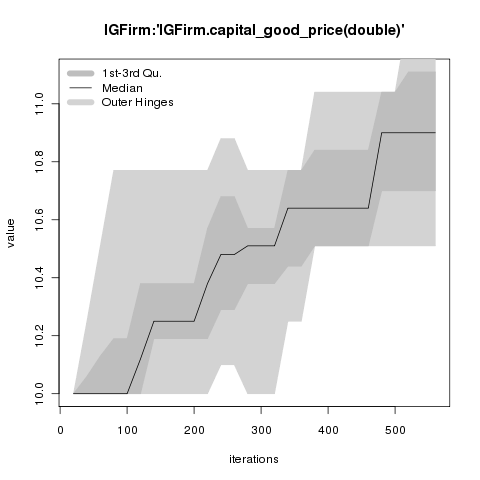
\includegraphics[width=6cm]{./png/duration_240/intensity_0.05/frequency_20/IGFirm-capital_good_price.png}
\includegraphics[width=6cm]{./png/duration_240/intensity_0.05/frequency_20/IGFirm-energy_costs_per_day.png}
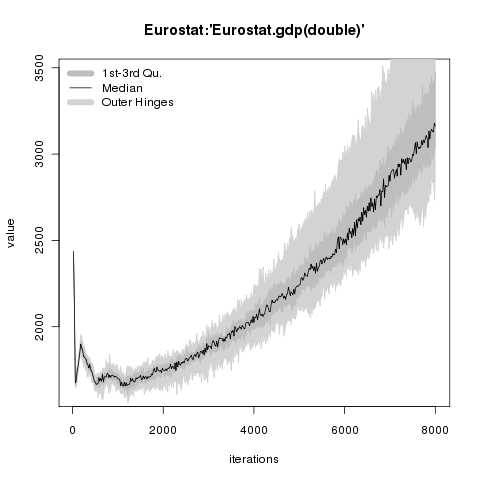
\includegraphics[width=6cm]{./png/duration_240/intensity_0.05/frequency_20/Eurostat-gdp.png}
\includegraphics[width=6cm]{./png/duration_240/intensity_0.05/frequency_20/Eurostat-unemployment_rate.png}
\end{minipage}
%\caption{Energy shock parameters: duration $d=240$, intensity $\pi=0.05, periodicity $\Pi=20$.}
%\label{Figure: IGFirm-capital_good_price}
\end{figure}


\pagebreak

%\subsubsection*{Duration $40$, intensity $5\%$, frequency $\{0,20,60\}$}
\begin{figure}[ht!]
\centering\leavevmode
\begin{minipage}{13cm}
\centering\leavevmode
{$d=240, \pi=0.05, \Pi=20$}\\
\includegraphics[width=6cm]{./png/duration_240/intensity_0.05/frequency_20/IGFirm-capital_good_price.png}
\includegraphics[width=6cm]{./png/duration_240/intensity_0.05/frequency_20/IGFirm-energy_costs_per_day.png}
\includegraphics[width=6cm]{./png/duration_240/intensity_0.05/frequency_20/Eurostat-gdp.png}
\includegraphics[width=6cm]{./png/duration_240/intensity_0.05/frequency_20/Eurostat-unemployment_rate.png}
\end{minipage}
%\caption{Energy shock parameters: duration $d=240$, intensity $\pi=0.05, periodicity $\Pi=20$.}
%\label{Figure: IGFirm-capital_good_price}
\end{figure}


\begin{figure}[ht!]
\centering\leavevmode
\begin{minipage}{13cm}
\centering\leavevmode
{$d=240, \pi=0.05, \Pi=20$}\\
\includegraphics[width=6cm]{./png/duration_240/intensity_0.05/frequency_20/IGFirm-capital_good_price.png}
\includegraphics[width=6cm]{./png/duration_240/intensity_0.05/frequency_20/IGFirm-energy_costs_per_day.png}
\includegraphics[width=6cm]{./png/duration_240/intensity_0.05/frequency_20/Eurostat-gdp.png}
\includegraphics[width=6cm]{./png/duration_240/intensity_0.05/frequency_20/Eurostat-unemployment_rate.png}
\end{minipage}
%\caption{Energy shock parameters: duration $d=240$, intensity $\pi=0.05, periodicity $\Pi=20$.}
%\label{Figure: IGFirm-capital_good_price}
\end{figure}


%\begin{figure}[ht!]
\centering\leavevmode
\begin{minipage}{13cm}
\centering\leavevmode
{$d=240, \pi=0.05, \Pi=20$}\\
\includegraphics[width=6cm]{./png/duration_240/intensity_0.05/frequency_20/IGFirm-capital_good_price.png}
\includegraphics[width=6cm]{./png/duration_240/intensity_0.05/frequency_20/IGFirm-energy_costs_per_day.png}
\includegraphics[width=6cm]{./png/duration_240/intensity_0.05/frequency_20/Eurostat-gdp.png}
\includegraphics[width=6cm]{./png/duration_240/intensity_0.05/frequency_20/Eurostat-unemployment_rate.png}
\end{minipage}
%\caption{Energy shock parameters: duration $d=240$, intensity $\pi=0.05, periodicity $\Pi=20$.}
%\label{Figure: IGFirm-capital_good_price}
\end{figure}


\pagebreak

%\subsubsection*{Duration $40$, intensity $10\%$, frequency $\{0,20,60\}$}
\begin{figure}[ht!]
\centering\leavevmode
\begin{minipage}{13cm}
\centering\leavevmode
{$d=240, \pi=0.05, \Pi=20$}\\
\includegraphics[width=6cm]{./png/duration_240/intensity_0.05/frequency_20/IGFirm-capital_good_price.png}
\includegraphics[width=6cm]{./png/duration_240/intensity_0.05/frequency_20/IGFirm-energy_costs_per_day.png}
\includegraphics[width=6cm]{./png/duration_240/intensity_0.05/frequency_20/Eurostat-gdp.png}
\includegraphics[width=6cm]{./png/duration_240/intensity_0.05/frequency_20/Eurostat-unemployment_rate.png}
\end{minipage}
%\caption{Energy shock parameters: duration $d=240$, intensity $\pi=0.05, periodicity $\Pi=20$.}
%\label{Figure: IGFirm-capital_good_price}
\end{figure}


\begin{figure}[ht!]
\centering\leavevmode
\begin{minipage}{13cm}
\centering\leavevmode
{$d=240, \pi=0.05, \Pi=20$}\\
\includegraphics[width=6cm]{./png/duration_240/intensity_0.05/frequency_20/IGFirm-capital_good_price.png}
\includegraphics[width=6cm]{./png/duration_240/intensity_0.05/frequency_20/IGFirm-energy_costs_per_day.png}
\includegraphics[width=6cm]{./png/duration_240/intensity_0.05/frequency_20/Eurostat-gdp.png}
\includegraphics[width=6cm]{./png/duration_240/intensity_0.05/frequency_20/Eurostat-unemployment_rate.png}
\end{minipage}
%\caption{Energy shock parameters: duration $d=240$, intensity $\pi=0.05, periodicity $\Pi=20$.}
%\label{Figure: IGFirm-capital_good_price}
\end{figure}


%\begin{figure}[ht!]
\centering\leavevmode
\begin{minipage}{13cm}
\centering\leavevmode
{$d=240, \pi=0.05, \Pi=20$}\\
\includegraphics[width=6cm]{./png/duration_240/intensity_0.05/frequency_20/IGFirm-capital_good_price.png}
\includegraphics[width=6cm]{./png/duration_240/intensity_0.05/frequency_20/IGFirm-energy_costs_per_day.png}
\includegraphics[width=6cm]{./png/duration_240/intensity_0.05/frequency_20/Eurostat-gdp.png}
\includegraphics[width=6cm]{./png/duration_240/intensity_0.05/frequency_20/Eurostat-unemployment_rate.png}
\end{minipage}
%\caption{Energy shock parameters: duration $d=240$, intensity $\pi=0.05, periodicity $\Pi=20$.}
%\label{Figure: IGFirm-capital_good_price}
\end{figure}


\pagebreak
\end{comment}

\begin{comment}
%\subsubsection*{Duration $240$, intensity $1\%$, frequency $\{0,20,60\}$}
\begin{figure}[ht!]
\centering\leavevmode
\begin{minipage}{13cm}
\centering\leavevmode
{$d=240, \pi=0.05, \Pi=20$}\\
\includegraphics[width=6cm]{./png/duration_240/intensity_0.05/frequency_20/IGFirm-capital_good_price.png}
\includegraphics[width=6cm]{./png/duration_240/intensity_0.05/frequency_20/IGFirm-energy_costs_per_day.png}
\includegraphics[width=6cm]{./png/duration_240/intensity_0.05/frequency_20/Eurostat-gdp.png}
\includegraphics[width=6cm]{./png/duration_240/intensity_0.05/frequency_20/Eurostat-unemployment_rate.png}
\end{minipage}
%\caption{Energy shock parameters: duration $d=240$, intensity $\pi=0.05, periodicity $\Pi=20$.}
%\label{Figure: IGFirm-capital_good_price}
\end{figure}


\begin{figure}[ht!]
\centering\leavevmode
\begin{minipage}{13cm}
\centering\leavevmode
{$d=240, \pi=0.05, \Pi=20$}\\
\includegraphics[width=6cm]{./png/duration_240/intensity_0.05/frequency_20/IGFirm-capital_good_price.png}
\includegraphics[width=6cm]{./png/duration_240/intensity_0.05/frequency_20/IGFirm-energy_costs_per_day.png}
\includegraphics[width=6cm]{./png/duration_240/intensity_0.05/frequency_20/Eurostat-gdp.png}
\includegraphics[width=6cm]{./png/duration_240/intensity_0.05/frequency_20/Eurostat-unemployment_rate.png}
\end{minipage}
%\caption{Energy shock parameters: duration $d=240$, intensity $\pi=0.05, periodicity $\Pi=20$.}
%\label{Figure: IGFirm-capital_good_price}
\end{figure}


\begin{figure}[ht!]
\centering\leavevmode
\begin{minipage}{13cm}
\centering\leavevmode
{$d=240, \pi=0.05, \Pi=20$}\\
\includegraphics[width=6cm]{./png/duration_240/intensity_0.05/frequency_20/IGFirm-capital_good_price.png}
\includegraphics[width=6cm]{./png/duration_240/intensity_0.05/frequency_20/IGFirm-energy_costs_per_day.png}
\includegraphics[width=6cm]{./png/duration_240/intensity_0.05/frequency_20/Eurostat-gdp.png}
\includegraphics[width=6cm]{./png/duration_240/intensity_0.05/frequency_20/Eurostat-unemployment_rate.png}
\end{minipage}
%\caption{Energy shock parameters: duration $d=240$, intensity $\pi=0.05, periodicity $\Pi=20$.}
%\label{Figure: IGFirm-capital_good_price}
\end{figure}


\pagebreak

%\subsubsection*{Duration $240$, intensity $5\%$, frequency $\{0,20,60\}$}
\begin{figure}[ht!]
\centering\leavevmode
\begin{minipage}{13cm}
\centering\leavevmode
{$d=240, \pi=0.05, \Pi=20$}\\
\includegraphics[width=6cm]{./png/duration_240/intensity_0.05/frequency_20/IGFirm-capital_good_price.png}
\includegraphics[width=6cm]{./png/duration_240/intensity_0.05/frequency_20/IGFirm-energy_costs_per_day.png}
\includegraphics[width=6cm]{./png/duration_240/intensity_0.05/frequency_20/Eurostat-gdp.png}
\includegraphics[width=6cm]{./png/duration_240/intensity_0.05/frequency_20/Eurostat-unemployment_rate.png}
\end{minipage}
%\caption{Energy shock parameters: duration $d=240$, intensity $\pi=0.05, periodicity $\Pi=20$.}
%\label{Figure: IGFirm-capital_good_price}
\end{figure}


\begin{figure}[ht!]
\centering\leavevmode
\begin{minipage}{13cm}
\centering\leavevmode
{$d=240, \pi=0.05, \Pi=20$}\\
\includegraphics[width=6cm]{./png/duration_240/intensity_0.05/frequency_20/IGFirm-capital_good_price.png}
\includegraphics[width=6cm]{./png/duration_240/intensity_0.05/frequency_20/IGFirm-energy_costs_per_day.png}
\includegraphics[width=6cm]{./png/duration_240/intensity_0.05/frequency_20/Eurostat-gdp.png}
\includegraphics[width=6cm]{./png/duration_240/intensity_0.05/frequency_20/Eurostat-unemployment_rate.png}
\end{minipage}
%\caption{Energy shock parameters: duration $d=240$, intensity $\pi=0.05, periodicity $\Pi=20$.}
%\label{Figure: IGFirm-capital_good_price}
\end{figure}


\begin{figure}[ht!]
\centering\leavevmode
\begin{minipage}{13cm}
\centering\leavevmode
{$d=240, \pi=0.05, \Pi=20$}\\
\includegraphics[width=6cm]{./png/duration_240/intensity_0.05/frequency_20/IGFirm-capital_good_price.png}
\includegraphics[width=6cm]{./png/duration_240/intensity_0.05/frequency_20/IGFirm-energy_costs_per_day.png}
\includegraphics[width=6cm]{./png/duration_240/intensity_0.05/frequency_20/Eurostat-gdp.png}
\includegraphics[width=6cm]{./png/duration_240/intensity_0.05/frequency_20/Eurostat-unemployment_rate.png}
\end{minipage}
%\caption{Energy shock parameters: duration $d=240$, intensity $\pi=0.05, periodicity $\Pi=20$.}
%\label{Figure: IGFirm-capital_good_price}
\end{figure}


\pagebreak

%\subsubsection*{Duration $240$, intensity $10\%$, frequency $\{0,20,60\}$}
\begin{figure}[ht!]
\centering\leavevmode
\begin{minipage}{13cm}
\centering\leavevmode
{$d=240, \pi=0.05, \Pi=20$}\\
\includegraphics[width=6cm]{./png/duration_240/intensity_0.05/frequency_20/IGFirm-capital_good_price.png}
\includegraphics[width=6cm]{./png/duration_240/intensity_0.05/frequency_20/IGFirm-energy_costs_per_day.png}
\includegraphics[width=6cm]{./png/duration_240/intensity_0.05/frequency_20/Eurostat-gdp.png}
\includegraphics[width=6cm]{./png/duration_240/intensity_0.05/frequency_20/Eurostat-unemployment_rate.png}
\end{minipage}
%\caption{Energy shock parameters: duration $d=240$, intensity $\pi=0.05, periodicity $\Pi=20$.}
%\label{Figure: IGFirm-capital_good_price}
\end{figure}


\begin{figure}[ht!]
\centering\leavevmode
\begin{minipage}{13cm}
\centering\leavevmode
{$d=240, \pi=0.05, \Pi=20$}\\
\includegraphics[width=6cm]{./png/duration_240/intensity_0.05/frequency_20/IGFirm-capital_good_price.png}
\includegraphics[width=6cm]{./png/duration_240/intensity_0.05/frequency_20/IGFirm-energy_costs_per_day.png}
\includegraphics[width=6cm]{./png/duration_240/intensity_0.05/frequency_20/Eurostat-gdp.png}
\includegraphics[width=6cm]{./png/duration_240/intensity_0.05/frequency_20/Eurostat-unemployment_rate.png}
\end{minipage}
%\caption{Energy shock parameters: duration $d=240$, intensity $\pi=0.05, periodicity $\Pi=20$.}
%\label{Figure: IGFirm-capital_good_price}
\end{figure}


\begin{figure}[ht!]
\centering\leavevmode
\begin{minipage}{13cm}
\centering\leavevmode
{$d=240, \pi=0.05, \Pi=20$}\\
\includegraphics[width=6cm]{./png/duration_240/intensity_0.05/frequency_20/IGFirm-capital_good_price.png}
\includegraphics[width=6cm]{./png/duration_240/intensity_0.05/frequency_20/IGFirm-energy_costs_per_day.png}
\includegraphics[width=6cm]{./png/duration_240/intensity_0.05/frequency_20/Eurostat-gdp.png}
\includegraphics[width=6cm]{./png/duration_240/intensity_0.05/frequency_20/Eurostat-unemployment_rate.png}
\end{minipage}
%\caption{Energy shock parameters: duration $d=240$, intensity $\pi=0.05, periodicity $\Pi=20$.}
%\label{Figure: IGFirm-capital_good_price}
\end{figure}


\end{comment}

%\end{document}

%\end{comment}

\chapter{Macroeconomic stabilization policies}
\section{Introduction}

In this section we focus on the use of subsidies to mitigate the negative
effects of shocks to the macroeconomy, in particular due to energy shocks.
Specifically, we introduce household subsidies and firm subsidies. These
subsidies are used to counteract the effects of the energy shock on the GDP
growth rate, unemployment and inflation by directly stimulating consumption,
employment and investment.

\bigskip The consumer subsidy is meant to compensate for the loss in
purchasing power of the households. The objective is to support the demand
side of the economy. Each household receives a subsidy as a percentage of
its total monthly consumption expenditure. This scheme is somewhat similar
to the US tax rebate implemented by G.W. Bush. The percentage is determined
at the end of each year, after the government has computed the current GDP
growth rate. The Government then announces this percentage, the agents
truthfully compute the total subsidy they shall receive and send a message
to the Government to claim it. The individual subsidies are computed at the
end of each month, after the households knows their total consumption
expenditures for the month. This scheme is equivalent to a negative VAT, and
amounts to a price discount.

\bigskip The consumer subsidy is activated as a function of the GDP growth
rate $X$, using two trigger levels $a$ and $b,$ with typically $a<b$. The
level $a$ is the `on' trigger, and $b$ the `off' trigger: 
The subsidy becomes active whenever the GDP growth rate \textit{falls} below $a$ ($%
X<a)$, and becomes inactive when the growth rate is again above $b$ ($X>b)$.

\bigskip The first level $a$ can be positive or negative. For example, an
aggressive stabilization policy might be to set this level to $a=0.03$
implying that the subsidy regime becomes active if the GDP growth rate drops
below $+3\%$. If instead $a=-0.01,$ the subsidy takes effect only after the
growth rate has fallen to -$1\%$. In both cases, as already mentioned, the
subsidy is awarded until $X$ increases to $b$. A justification for the
asymmetry between the on and off triggers is that the subsidy typically gets
activated relatively late during a downturn because of recognition,
decision, and implementation lags, but should remain active until strong
growth is assured again.

\bigskip The magnitude $S$ of the subsidy is given by:
\begin{equation}
\begin{array}{l}
S=-|X|\tanh (X-b).\text{ }%
\end{array}%
\end{equation}

\begin{figure}[ht!]
\centering\leavevmode
\begin{boxedminipage}{14cm}
\centering\leavevmode
\includegraphics[width=8cm]{./stabilization/png/subsidy.png}
\end{boxedminipage}
\caption{Graph of the subsidy multiplication factor $s$. To obtain the
actual subsidy this should be multiplied by $|X|$.}
\label{Figure: subsidy multiplication factor}
\end{figure}

In the case of the firm, the subsidy is meant to compensate the firm for an
increase in production costs. These costs consist of labour costs and the
costs of acquiring new capital. Therefore we can use the firm's total
investments as a basis for the subsidy. Firms compute the subsidy amount
truthfully at the end of their subjective month, after they have computed
their capital investments, and send a message to the government informing it
of the amount to be paid.
 %1.5 pages
\clearpage
\pagebreak
\pagebreak

\section{Simulation results}
We consider the worst case scenario of a prolonged energy crisis with $12$ cumulative shocks of $5\%$ ($d=240$, $\pi=0.05$, $\Pi=20$).
Figure \ref{Figure: energy shock 4 growth} shows the GDP growth rate during the energy crisis of the previous section. 

As discussed in the experimental design, we need to set the trigger for the policy.
The first trigger we set to $-5\%$, which means that the subsidy will not take effect until the annualized growth rate of GDP falls below $-5\%$. Note that the government in our model only detects this trigger once a year, so it really has to be a sustained economic downturn before the policy takes effect. In the example the subsidy would be activated around iteration 1200, when the economy first reaches below $-5\%$ growth.

The second trigger is set the $+5\%$ which in our example means that the subsidy would only be turned off at iteration 1600, when the economy starts to grow by more than $+5\%$ on a yearly basis. After that it never reaches below $-5\%$ again so the subsidy will remain inactive.

Figure \ref{Figure: Stabilization} shows the effect of the stabilizing subsidy. The growth rate is back to positive levels which is financed subsidy payments by the government.

\begin{figure}[ht!]
\centering\leavevmode
\begin{minipage}{17cm}
\centering\leavevmode
\includegraphics[width=8cm]{./energy_shock/png/duration_240/intensity_0.05/frequency_20/Eurostat-annual_growth_rates_monthly_gdp.png}
\end{minipage}
\caption{Growth rate of GDP during the energy crisis.}
\label{Figure: energy shock 4 growth}
\end{figure}

\begin{figure}[ht!]
\centering\leavevmode
\begin{minipage}{17cm}
\centering\leavevmode
%\includegraphics[width=8cm]{./energy_shock/png/duration_240/intensity_0.05/frequency_20/Eurostat-annual_growth_rates_monthly_gdp.png}
%\includegraphics[width=8cm]{./energy_shock/png/duration_240/intensity_0.05/frequency_20/Eurostat-total_subsidy_payment.png}
\end{minipage}
\caption{Effect of the stabilization policy in the energy shock experiment. Annualized growth rate and total subsidy payment by the government.}
\label{Figure: Stabilization}
\end{figure}
%\pagebreak 


\end{document} 